Na wykresie \ref{fig:JumpingValues} przedstawiono przykładowy przebieg wartości dla pierwszych 5 zmian
wraz z zaznaczonymi miejscami,
gdzie nastąpiła.
\begin{figure}[htbp]
  \centering
  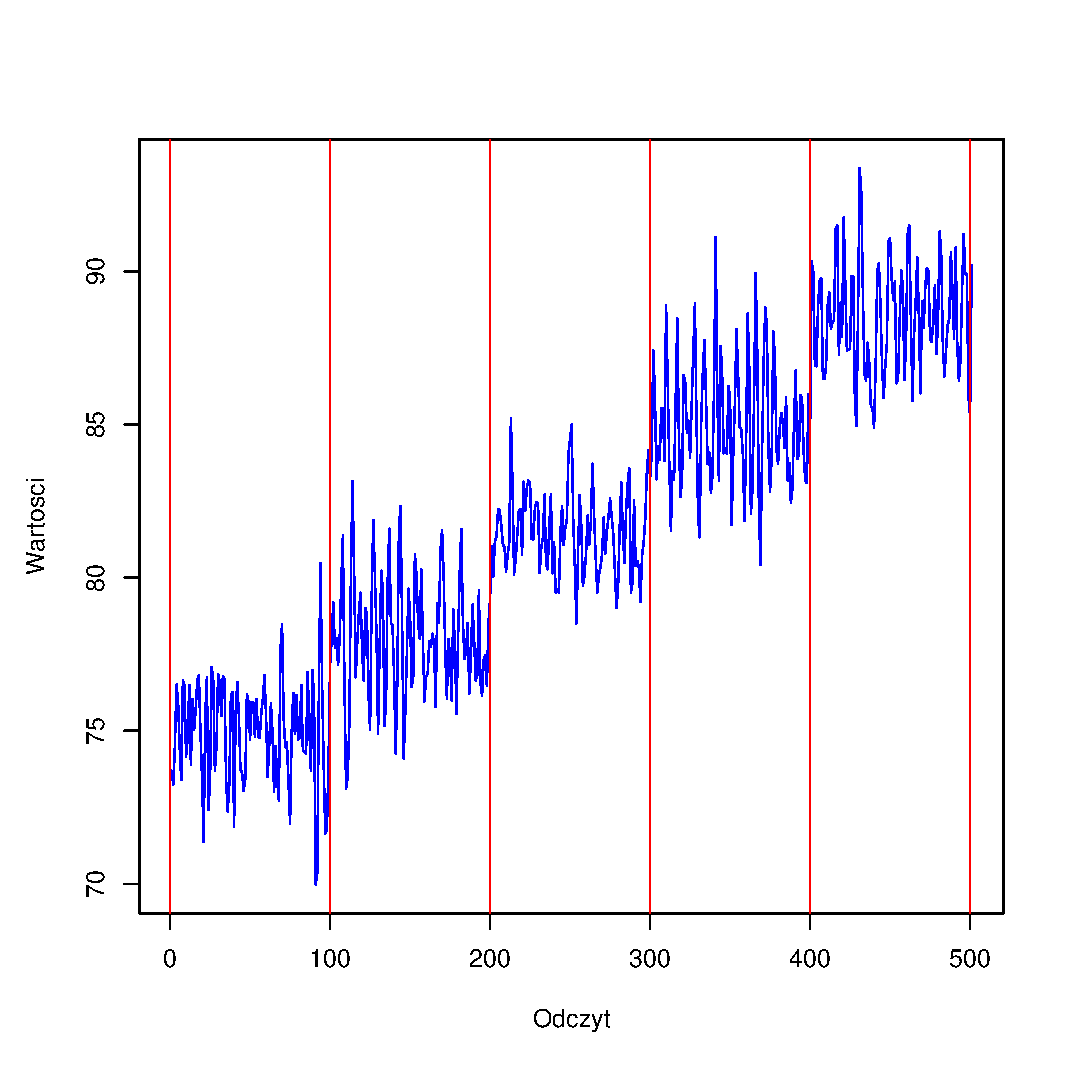
\includegraphics[width=0.8\textwidth]{img/ch-5-jumping}
  \caption{Przykładowe wartości}
  \label{fig:JumpingValues}
\end{figure}
Badanie przeprowadzono poprzez wygenerowanie 20 zestawów danych.
Źródło (\textit{seed}) dla każdego z zestawów były inne.
